\chapter{Context Survey}

This project aims to develop a framework for capturing the opinions of users. This closely aligns with the idea of gamifying surveys - a concept that is introduced in section \ref{surgam}. Section \ref{soft} describes software that attempts to fulfil a similar role to OpDeck, analysing their various strengths and weaknesses.

\section{Survey Gamification}\label{surgam}
An emerging trend in modern business practice, \textit{gamification} can be defined as `using game mechanics and game design elements to measure, influence and reward user behaviors.'~\cite{7804551}. 
There has been some research into gamification as a tool to improve the quality of responses from and engagement with surveys. From this I aim to gain an awareness of the necessary considerations when designing and implementing gamification.

As of yet, most experiments into survey gamification have only gone so far as to change the wording of survey questions, show questions alongside imagery or change the answer input mechanics.
My project represents a considerable departure from the standard survey format, with the goal being that the game could be enjoyed as a standalone experience. 
Because of this, there are many psychological considerations as to the validity of the results that can be gathered through this format. 
There exists a tradeoff between complex levels of gamificaiton that increase enjoyment, and the accuracy of respondent data. 
It is also difficult to be certain whether player's will respond the same way in a game as they would in real life.
While deep investigation of these issues is not my goal, I deemed it important to understand them, in an attempt to minimise any bias that my framework could impose onto players.

A 2011 paper found that while participants' enjoyment of the survey is generally increased, there are three main aspects of gamification that can affect the `character of the data'~\cite{GameExperiments}:
\begin{enumerate}[label=\textbf{e.\arabic*}]
    \item\label{cd:q} Effects caused by changes to the question and how it is interpreted
    \item\label{cd:m} Effects caused by changing the attitude and mindset of respondents
    \item\label{cd:l} Effects caused by changes to the design and layout of question
\end{enumerate}
These considerations are targeted towards those gamified surveys that still have a fairly standard format - I do however believe that they are still applicable to my project. 

A key aspect of the framework I designed is the context that is persistent between questions, and affected by player's choices. Harms \etal wrote in a 2015 paper~\cite{Olympic} that `Designers may also implement feedback loops, i.e., dynamics wherein user actions affect the overall state of gameplay. Feedback loops may visualize concepts such as a user’s progress, status, wealth, health, points, etc.'. 
This gives me confidence that adding a persistent context to the game is a valid design decision.
As for how this will affect the character of the data, I believe this relates to~\ref{cd:q}. 
This is because changing the context effectively changes the question, as people may respond differently under different circumstances. 

\ref{cd:l} will also occurr in my artifact - where there is a UI to interact with, there is potential to influence the way the user interacts with it. I will attempt to minimise this risk - ideally the only bias imposed on a player's decision will be from the game definition itself.

Brownell \etal \cite{SurveyGamificationResearch} summarise the state of research into survey gamification as follows:
`In most cases, their results show that the addition of these game elements increases the length and quantity of responses, and respondents typically prefer the gamified version to the standard survey version. However, their research does not compare the effectiveness of game elements in gamified surveys. They have also found that that some gamified survey designs can lead to compromised respondent data (Puleston \& Sleep, 2011).'~\cite{SurveyGamificationResearch}.
This indicates that there is promise in the notion of gamifying surveys - however it can result in a reduction in accuracy of the data collected. Depending on the extent to which the survey is abstracted from, precise details, both of the question and response, can be lost. Given this, gamification is likely best suited to situations in which the surveyors need broad answers, rather than precise ones.

\section{Similar Software}\label{soft}

\subsection{Datagame}
Datagame~\cite{Datagame} is a company that offers services allowing researchers to create and publish gamified surveys. This is done through interfaces that are heavily game-influenced, such as word searches and decks of cards.

Datagame supplies the tools required to populate one of several template games with custom questions, and export this to an online format that can be played through many channels including Facebook~\cite{Facebook}. 

Datagame offer four game types available to customise. The one most similar to the game I intend to create is referred to as a `Swiper' game. In this, the player draws cards from a virtual deck, each of which presents a yes/no question. The user swipes the card left or right to answer yes or no respectively. Figure~\ref{fig:datagame} shows this interface - it is fairly simple, with no standout features other than those added during configuration. Customisation options include allowing the user to replace card backgrounds with images, as well as change the colour of the text. Figure~\ref{fig:dg_editor} shows an example of the game editing view in which the following aspects of the game can be edited:

\begin{itemize}
    \item Project title
    \item Title question
    \item List of cards
    \item Card name
    \item Card text/images
    \item Toggle card shuffling
    \item Game UI labels
    \item Background image
\end{itemize}

\begin{figure}[!h]
	\centering
	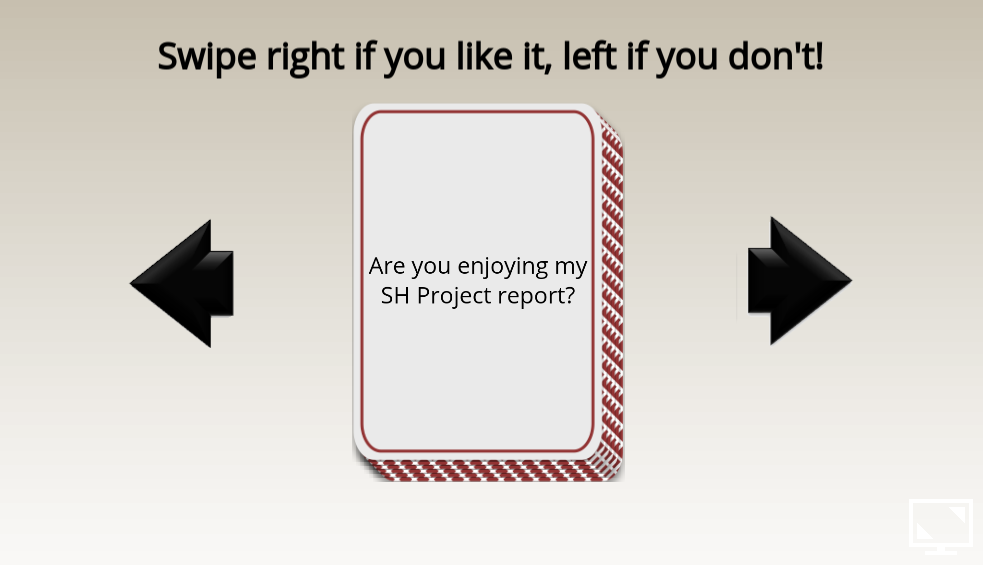
\includegraphics[width=0.9\textwidth]{./images/context/datagame.png}
	\caption{Example question in one of the Datagame~\cite{Datagame} game types, which involves answering yes or no questions by swiping left or right.}
	\label{fig:datagame}
\end{figure}

\begin{figure}[!h]
	\centering
	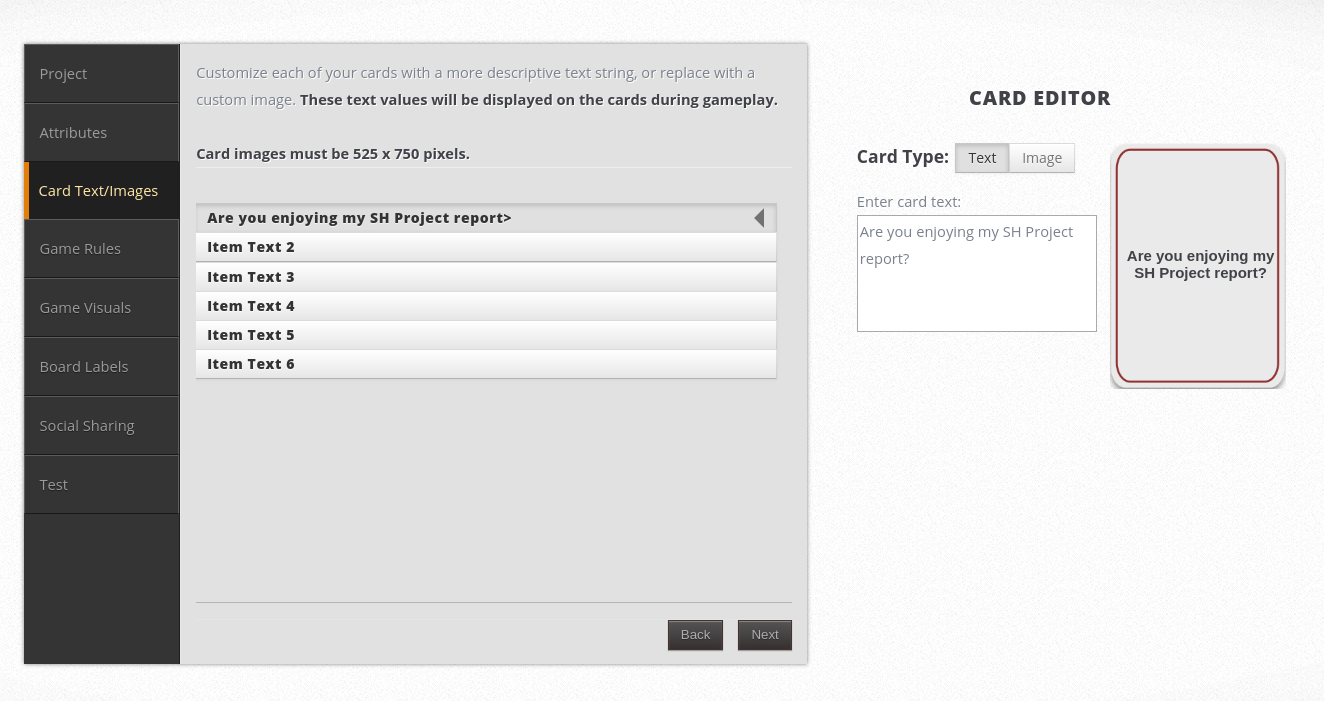
\includegraphics[width=0.9\textwidth]{./images/context/dg_editor.png}
	\caption{Process of editing the Datagame~\cite{Datagame} game instance shown in figure~\ref{fig:datagame}.}
	\label{fig:dg_editor}
\end{figure}

This format excels in allowing participants to answer a high volume of questions in a short space of time. 
The participant is asked questions directly, therefore there should be no ambiguity in their understanding beyond the wording of individual questions. 
The limitation of a binary choice reduces the precision with which the player can answer the given question - this may be acceptable for only a subset of surveys that don't require precise answers.
While the interface has the appearance of a game, the gameplay elements are shallow. 
There is no conditional branching in this game, as cards can only be removed by answering them and there is no way to add cards to the deck during a game. 
Further, the participant's responses have no observable consequences on the future of the game, and there is no goal. This leaves the user with little incentive to continue playing beyond the appearance of the interface, and the content of the questions themselves.

Given the above, while Datagame surveys are presented as games, they are merely a wrapper around a traditional binary choice survey format.

\subsection{Qualifio}
Qualifio~\cite{Qualifio} offer a similar service, providing a larger variety of game formats than Datagame. 
I was not able to access Qualifio's game creation tools, as this functionality is behind a paywall, however the site does host playable examples. 
Qualifio's toolset features the `Swiper' style game seen in figure \ref{fig:qual} which, from the perspective of the participant, is very similar to that provided by Datagame. This comes with the same tradeoff between engagement, accuracy of results and precision of input.

\begin{figure}[!h]
	\centering
	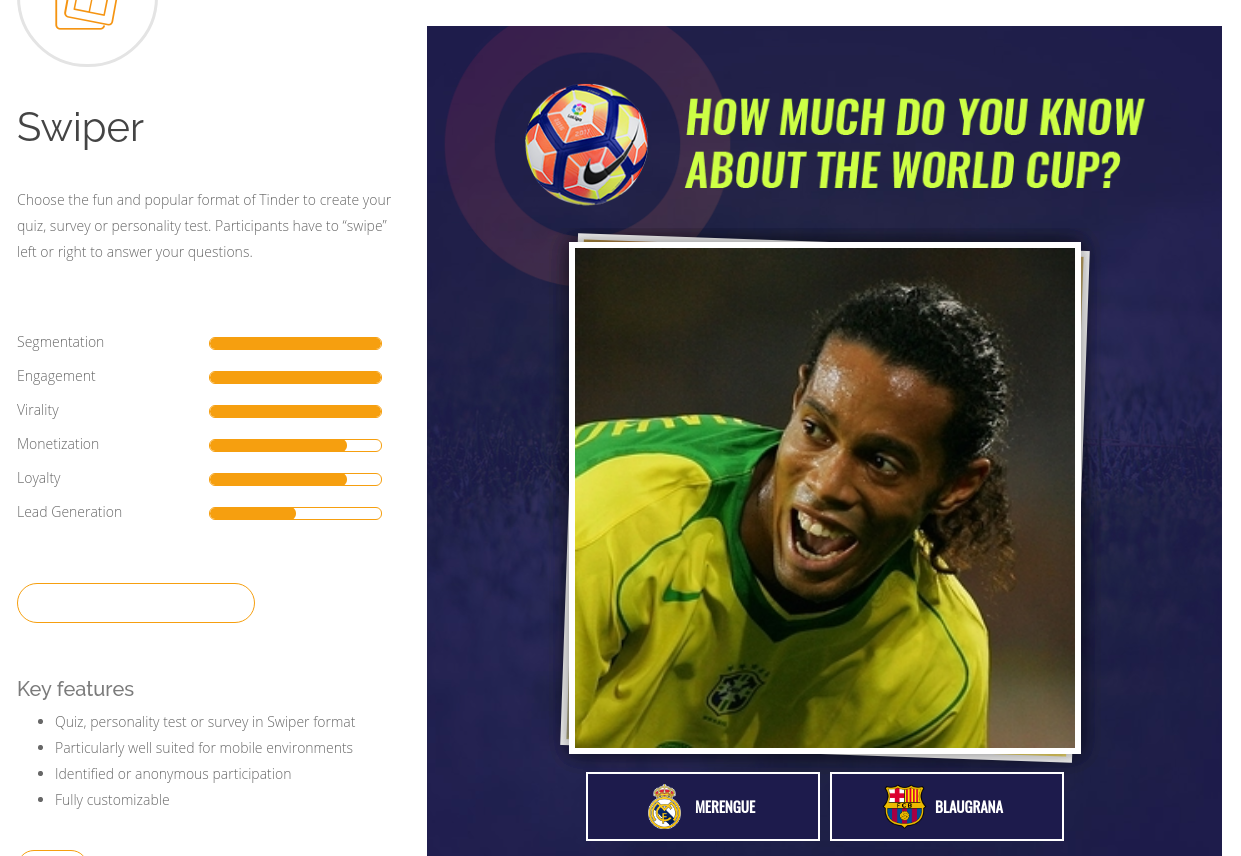
\includegraphics[width=0.9\textwidth]{./images/context/qual.png}
	\caption{Qualifio~\cite{Qualifio} swiper demo. This example game has players swipe or click depending on which team they think a given football player belongs to.}
	\label{fig:qual}
\end{figure}

Figure~\ref{fig:unit} shows another type of data collection game offered by Qualifio called `Ranking'. 
This offers a different approach to gathering user opinions, where multiple options are ranked in order of preference.
This is done through a click and drag interface, which is more engaging than the pen and paper equivalent of labelling each option with a rank number. 

\begin{figure}[!h]
	\centering
	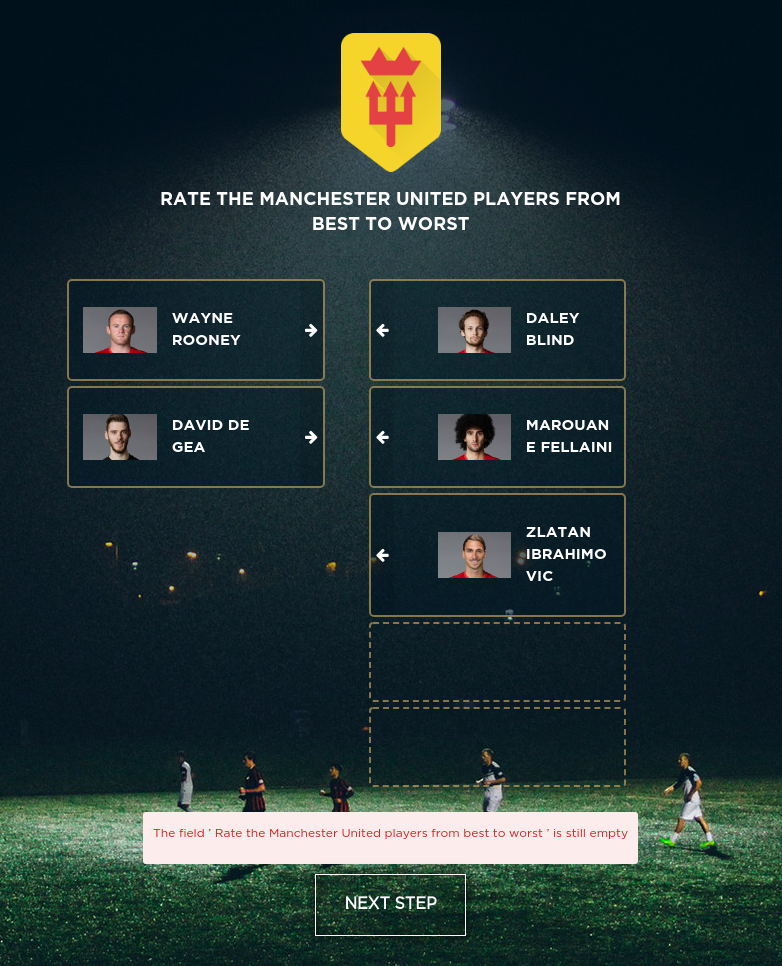
\includegraphics[width=0.9\textwidth]{./images/context/united.png}
	\caption{Qualifio~\cite{Qualifio} Ranking demo. This example has players rank football players from top to bottom - best to worst.}
	\label{fig:unit}
\end{figure}

Ranking gives users more precision in their answers than is available with Swiper, however the results are all relative to each other. If one user likes all of the options, and another dislikes them all, it's possible that they will have the same answer - the absolute values are lost in place of relative data.

Figures~\ref{fig:check} and~\ref{fig:pred} show examples of other games that Qualifio offer.

\begin{figure}[!h]
	\centering
	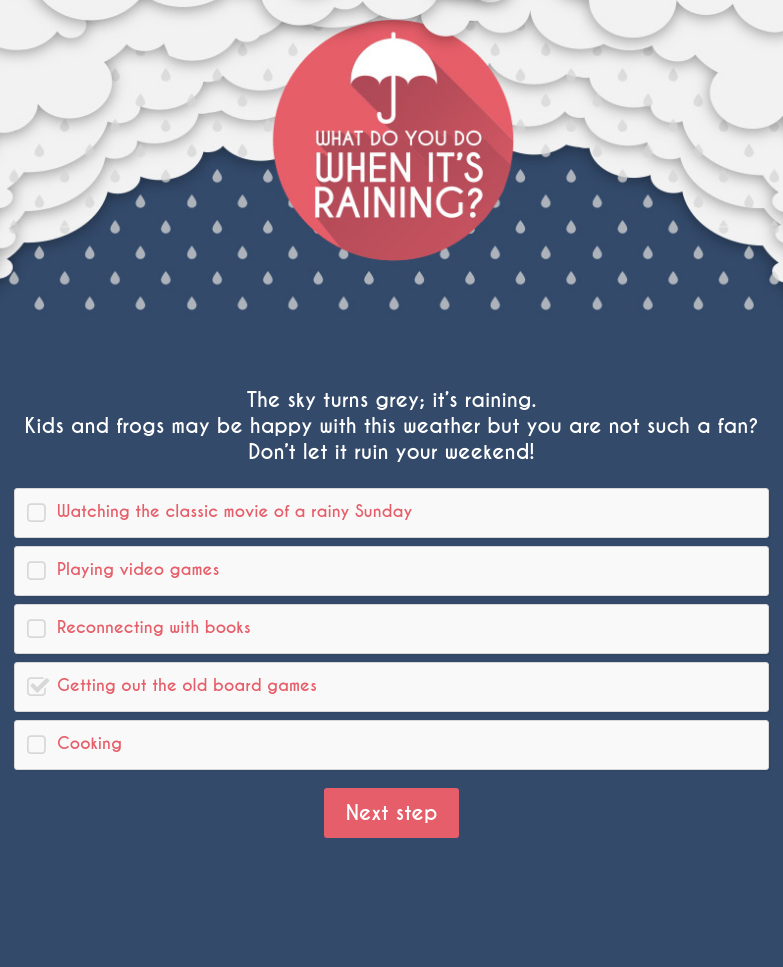
\includegraphics[width=0.9\textwidth]{./images/context/check.png}
	\caption{Qualifio~\cite{Qualifio} Checklist demo. Players check answers that they agree with.}
	\label{fig:check}
\end{figure}

The prediction game in figure \ref{fig:pred} provides an example of a game format that targets a specific category of questions - what players predict the result of an upcoming competition will be.

\begin{figure}[!h]
	\centering
	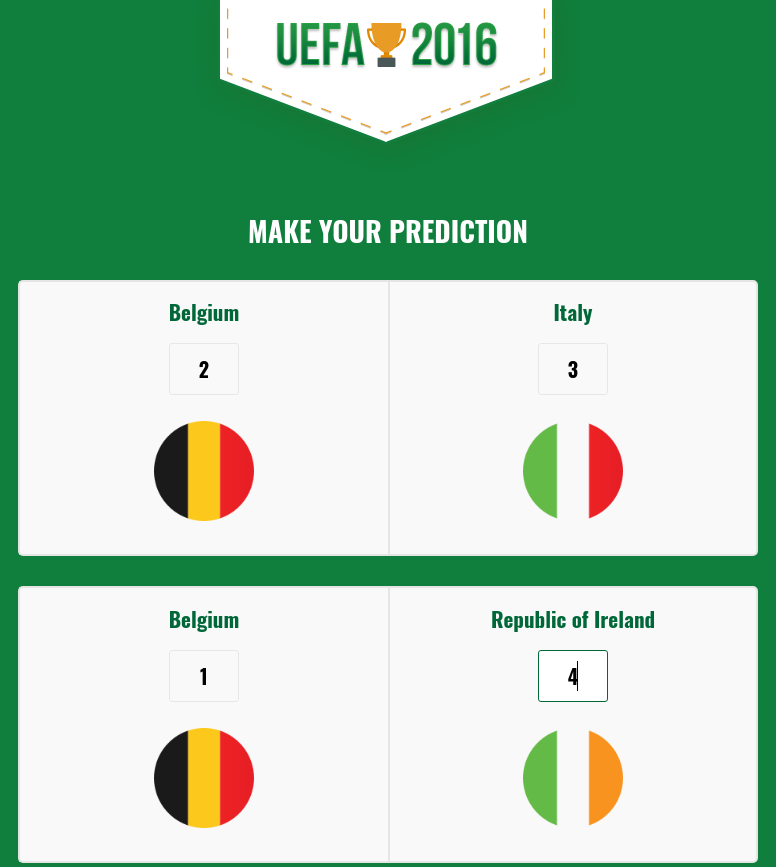
\includegraphics[width=0.9\textwidth]{./images/context/pred.png}
	\caption{Qualifio~\cite{Qualifio} Prediction demo. Players predict the scores of two parties.}
	\label{fig:pred}
\end{figure}

\subsection{Reigns}
Reigns is a multi-platform game in which the player takes the role of a medieval ruler, making binary decisions to solve problems their subjects approach them with. 
These decisions affect which scenarios may later appear, as well as changing how the ruler is perceived by various factions, such as their population, army, and church. 
The player's success is measured by how many decisions they can make without falling out of favour with any of the factions.

Reigns markets itself purely as a game, with no data-collecting functionality. In addition, the framework on which it is built is proprietary, so it is not possible to design scenarios around topics of interest. For these reasons, it cannot reasonably be used to collect and analyse data from players' choices. 

As of 2019-03-01, Reigns is a well reviewed game, with a rating of 4.7/5 on the Google Play store~\cite{GooglePlay}.
Building an intuitive game maker interface similar to that of Datagame~\cite{Datagame} along with portals through which these games can be played and analysed has the potential to make rich gamification of user opinion surveys accessible to researchers.
